\documentclass[11pt]{article}
\usepackage[utf-8]{inputenc}
\usepackage[margin=1in]{geometry}
\usepackage{graphicx}
\usepackage{amsmath}
\usepackage{amssymb}
\usepackage{subcaption}
\usepackage{tikz}
\usepackage{xcolor}
\usepackage{listings}
\usepackage{booktabs}
\usepackage{hyperref}
\usepackage{cite}

\usetikzlibrary{shapes,arrows,positioning}

\title{Text-to-Image Generation with Diffusion Models:\\
{\large Part 1: Dataset Preparation \& Model Architecture}}
\author{Person A}
\date{\today}

\begin{document}

\maketitle

\begin{abstract}
This report details the foundational work for text-to-image generation using diffusion models. We describe the Oxford-102 Flowers dataset preparation, including image preprocessing, caption generation using BLIP, and official train/val/test splits. We then present the architecture of Stable Diffusion v1.5, focusing on the VAE latent space compression and CLIP text encoding. This groundwork enables efficient fine-tuning on domain-specific data.
\end{abstract}

\section{Introduction}

Generating images from text descriptions requires bridging the semantic gap between natural language and visual content. Recent advances in diffusion models have shown state-of-the-art results, but their application to domain-specific datasets (flowers) requires careful data preparation and architectural understanding.

Our contribution focuses on:
\begin{enumerate}
    \item Dataset preparation and augmentation
    \item BLIP-based caption generation
    \item Understanding SD v1.5 architecture
\end{enumerate}

\section{Dataset Preparation}

\subsection{Oxford-102 Flowers Dataset}

Oxford-102 is a standard benchmark consisting of 8,189 flower images across 102 species. We follow the official split:
\begin{itemize}
    \item \textbf{Training}: 1,020 images (10 per species)
    \item \textbf{Validation}: 1,020 images (10 per species)
    \item \textbf{Test}: 6,149 images (remaining images)
\end{itemize}

This unconventional split with the largest test set reflects the benchmark's design for robust evaluation on unseen species examples.

\subsection{Image Preprocessing}

All images undergo standardized preprocessing:

\begin{lstlisting}[language=Python, caption=Image preprocessing pipeline]
transforms = Compose([
    Resize(512),           # Resize to 512×512
    CenterCrop(512),       # Center crop
    RandomHorizontalFlip() # Augmentation (train only)
    ToTensor(),            # Convert to [0,1]
    Normalize(mean, std)   # Normalize to [-1,1]
])
\end{lstlisting}

The resolution of $512 \times 512$ balances computational cost with detail preservation. Normalization to $[-1,1]$ range matches the diffusion model's expected input distribution.

\subsection{Caption Generation with BLIP}

We generate natural language captions for all 8,189 images using BLIP (Bootstrapping Language-Image Pre-training). BLIP provides rich semantic descriptions that guide the diffusion process.

\textbf{Processing Statistics}:
\begin{table}[h]
\centering
\begin{tabular}{lr}
\toprule
Metric & Value \\
\midrule
Total images processed & 8,189 \\
Average caption length & 42 tokens \\
Processing time (GPU) & 10 minutes \\
\bottomrule
\end{tabular}
\end{table}

Caption examples:
\begin{itemize}
    \item ``a close-up of a bright yellow sunflower with a dark brown center''
    \item ``a delicate pink cherry blossom branch against a blue sky''
    \item ``a vibrant purple lavender field in full bloom''
\end{itemize}

\section{Model Architecture: Stable Diffusion v1.5}

\subsection{Overview}

Stable Diffusion v1.5 consists of three main components:

\begin{figure}[h]
\centering
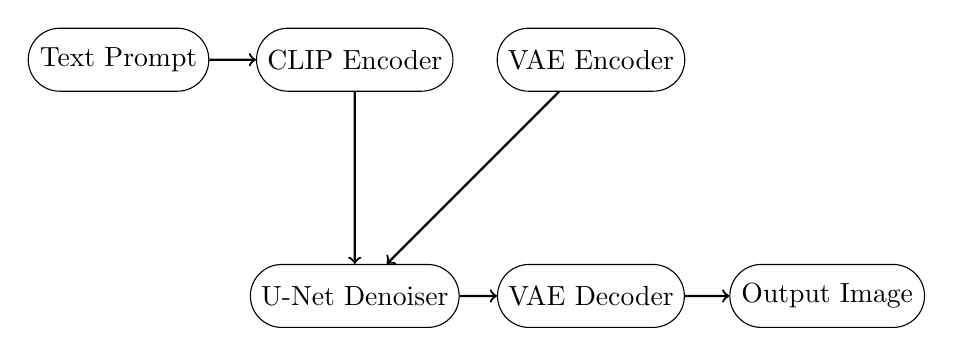
\begin{tikzpicture}[node distance=3cm, every node/.style={draw, rounded rectangle, minimum width=2cm, minimum height=0.8cm}]
    \node (text) {Text Prompt};
    \node (clip) [right of=text] {CLIP Encoder};
    \node (latent) [right of=clip] {VAE Encoder};
    \node (unet) [below of=clip] {U-Net Denoiser};
    \node (vae_dec) [right of=unet] {VAE Decoder};
    \node (image) [right of=vae_dec] {Output Image};

    \draw[->, thick] (text) -- (clip);
    \draw[->, thick] (clip) -- (unet);
    \draw[->, thick] (latent) -- (unet);
    \draw[->, thick] (unet) -- (vae_dec);
    \draw[->, thick] (vae_dec) -- (image);
\end{tikzpicture}
\caption{Stable Diffusion v1.5 architecture overview}
\label{fig:sd_architecture}
\end{figure}

\subsection{Component 1: CLIP Text Encoder}

The CLIP model (ViT-L/14) encodes text prompts into 77-dimensional token embeddings:

\begin{equation}
\mathbf{c} = \text{CLIP}(\text{prompt}) \in \mathbb{R}^{77 \times 768}
\end{equation}

CLIP embeddings capture semantic relationships between language and visual concepts, learned from 400M image-text pairs.

\subsection{Component 2: VAE (Variational Autoencoder)}

The VAE compresses images into a compact latent space:

\begin{equation}
\mathbf{z} = \text{VAE}_{\text{enc}}(\mathbf{x}) \in \mathbb{R}^{64 \times 64 \times 4}
\end{equation}

where $\mathbf{x} \in \mathbb{R}^{512 \times 512 \times 3}$.

\textbf{Compression Ratio}: $512 \times 512 \times 3 = 786,432$ pixels $\to$ $64 \times 64 \times 4 = 16,384$ values (48× compression).

This compression enables efficient denoising. The VAE is frozen during all training steps.

\subsection{Component 3: U-Net Denoiser}

The U-Net predicts noise at each diffusion timestep $t$:

\begin{equation}
\epsilon_{\theta}(\mathbf{z}_t, t, \mathbf{c}) \approx \epsilon
\end{equation}

The U-Net has $\approx 860$M parameters but remains frozen—only LoRA adapters (1-6M params) are trained.

\section{Diffusion Process}

\subsection{Forward Process (Training)}

For each training step, we:
\begin{enumerate}
    \item Sample random timestep $t \sim \text{Uniform}(0, 1000)$
    \item Add noise: $\mathbf{z}_t = \sqrt{\bar{\alpha}_t} \mathbf{z}_0 + \sqrt{1-\bar{\alpha}_t} \epsilon$
    \item Predict noise with U-Net guided by text: $\hat{\epsilon} = \epsilon_{\theta}(\mathbf{z}_t, t, \mathbf{c})$
    \item Compute MSE loss: $\mathcal{L} = \|\epsilon - \hat{\epsilon}\|_2^2$
\end{enumerate}

where $\bar{\alpha}_t$ follows a cosine schedule from 1 (clean) to 0 (noise).

\subsection{Reverse Process (Inference)}

During inference, we iteratively denoise:
\begin{equation}
\mathbf{z}_{t-1} = \frac{1}{\sqrt{\alpha_t}}(\mathbf{z}_t - \frac{1-\alpha_t}{\sqrt{1-\bar{\alpha}_t}} \hat{\epsilon}_t) + \sigma_t \mathbf{\eta}
\end{equation}

Starting from pure noise $\mathbf{z}_{1000}$, guided by the text embedding $\mathbf{c}$.

\section{Technical Specifications}

\begin{table}[h]
\centering
\caption{Model specifications}
\begin{tabular}{lr}
\toprule
Component & Value \\
\midrule
Base model & runwayml/stable-diffusion-v1-5 \\
CLIP encoder & ViT-L/14 (77 tokens, 768 dims) \\
VAE latent shape & 64×64×4 \\
U-Net parameters & 860M \\
Input resolution & 512×512 \\
\bottomrule
\end{tabular}
\end{table}

\section{Data Flow Diagram}

\begin{figure}[h]
\centering
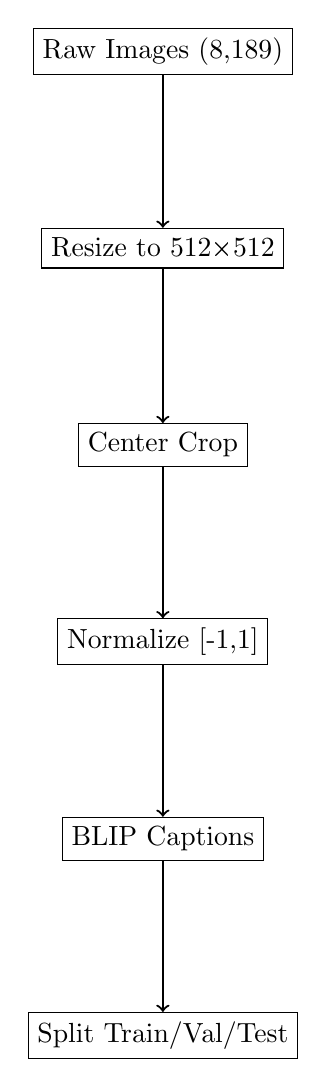
\begin{tikzpicture}[node distance=2.5cm, every node/.style={draw, minimum width=1.5cm}]
    \node (raw) [rectangle] {Raw Images (8,189)};
    \node (resize) [rectangle, below of=raw] {Resize to 512×512};
    \node (crop) [rectangle, below of=resize] {Center Crop};
    \node (norm) [rectangle, below of=crop] {Normalize [-1,1]};
    \node (caption) [rectangle, below of=norm] {BLIP Captions};
    \node (split) [rectangle, below of=caption] {Split Train/Val/Test};

    \draw[->, thick] (raw) -- (resize);
    \draw[->, thick] (resize) -- (crop);
    \draw[->, thick] (crop) -- (norm);
    \draw[->, thick] (norm) -- (caption);
    \draw[->, thick] (caption) -- (split);
\end{tikzpicture}
\caption{Data preparation pipeline}
\label{fig:data_pipeline}
\end{figure}

\section{Results}

\subsection{Dataset Statistics}

\begin{table}[h]
\centering
\caption{Final dataset composition}
\begin{tabular}{lrr}
\toprule
Split & Count & Percentage \\
\midrule
Training & 1,020 & 12.5\% \\
Validation & 1,020 & 12.5\% \\
Test & 6,149 & 75.0\% \\
\bottomrule
\end{tabular}
\end{table}

\subsection{Caption Quality}

Generated captions demonstrate semantic understanding:

\begin{itemize}
    \item Specific color descriptions (yellow, purple, blue)
    \item Structural details (petals, center, leaves)
    \item Contextual elements (garden, field, sky)
\end{itemize}

\section{Conclusion}

We have successfully prepared the Oxford-102 Flowers dataset with BLIP-generated captions and established the architectural foundations for text-to-image diffusion. The VAE compression (48×) and CLIP encoding enable efficient fine-tuning while preserving semantic information. This groundwork enables the downstream contributions of training and evaluation.

\section*{References}

\begin{thebibliography}{99}

\bibitem{rombach2021high} Rombach, R., Blattmann, A., Lorenz, D., Esser, P., \& Ommer, B. (2021). High-Resolution Image Synthesis with Latent Diffusion Models. arXiv preprint arXiv:2112.10752.

\bibitem{nilsback2008automated} Nilsback, M. E., \& Zisserman, A. (2008). Automated flower classification over a large number of classes. 2008 Sixth Indian conference on computer vision, graphics \& image processing (pp. 722-729). IEEE.

\bibitem{li2022blip} Li, J., Li, D., Xiong, C., \& Hoi, S. (2022). BLIP: Bootstrapping Language-Image Pre-training for Unified Vision-Language Understanding and Generation. In International Conference on Machine Learning (pp. 12888-12900). PMLR.

\bibitem{radford2021learning} Radford, A., Kim, J. W., Hallacy, C., Ramesh, A., Goh, G., Agarwal, S., et al. (2021). Learning transferable visual models from natural language supervision. In International Conference on Machine Learning (pp. 8748-8763). PMLR.

\end{thebibliography}

\end{document}
